\documentclass[11pt]{article}
\usepackage{amssymb, amsmath, libertine, hyperref, xcolor, booktabs, enumitem, microtype}
\usepackage[T1]{fontenc}
\usepackage[margin=1in]{geometry}
\usepackage{tikz}
\definecolor{dark-red}{rgb}{0.4,0.15,0.15}
\definecolor{blue-g}{rgb}{0.15,0.28,0.45}
\hypersetup{colorlinks, linkcolor=dark-red, citecolor=dark-red, urlcolor=dark-red}
\setlist[enumerate,1]{label=\textbf{(\alph*)}, leftmargin=*, itemsep=6pt, topsep=5pt}
\pagestyle{empty}
\newcommand{\prob}[1]{\medskip\noindent\textbf{\large #1}\par\smallskip}
\begin{document}

\begin{center}
{\Large\bfseries Math 111: Calculus \quad Homework 5}\\[4pt]
{Due Friday, December 4 by 10:00\textsc{p.m.} via Gradescope}
\end{center}

\medskip
\noindent\textbf{Covers} Active Calculus \S6.1--\S6.4. Every problem uses the same move:
slice, approximate one slice, add, take the limit. Problems~1 and~2 use \S6.1 and \S6.2 and
can be done after Wednesday, November~25. Problem~3 uses \S6.3 (Monday, November~30);
Problem~4 uses \S6.4 (Wednesday, December~2). The antiderivative reference sheet from
Exam~3 is fair to use.

\smallskip
\noindent\textbf{Before you start.} Write in sentences and paragraphs, as an
explanation another student in this course could read and follow. Draw diagrams large
and label them. You are encouraged to work with classmates; cite everyone you worked
with, and write your solutions independently --- duplicated solutions are an Honor
Principle violation. Each problem is marked holistically on the 0--5 scale, with up
to two further points for the quality of the writing. If you need an extension, use
the \href{https://docs.google.com/forms/d/e/1FAIpQLSfIfgx44SFtUzefTNr-80yz35MVJaUqQttt96xVTU5mCQCOgg/viewform}{extension
form} \emph{before} the deadline.

\bigskip\hrule\bigskip
\prob{1. Slicing a region two ways, and two lengths}
Let $R$ be the region between the curves $y=\sqrt x$ and $y=\frac x2$, shaded below.
\begin{center}
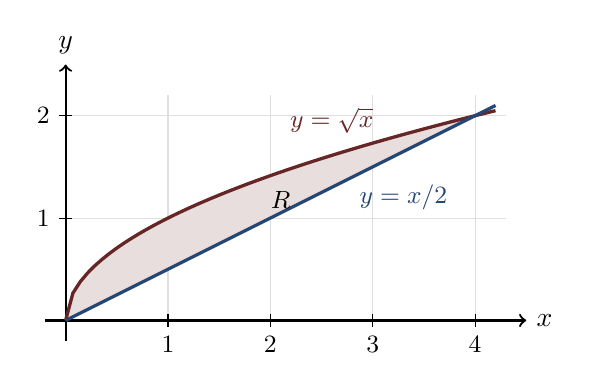
\begin{tikzpicture}[x=1.3cm,y=1.3cm]
  \foreach \gX in {0,...,4} \draw[gray!25] (\gX,0) -- (\gX,2.2);
  \foreach \gY in {0,1,2} \draw[gray!25] (0,\gY) -- (4.3,\gY);
  \fill[dark-red!15, domain=0:4, samples=60] plot (\x,{sqrt(\x)}) -- (4,2) -- plot[domain=4:0] (\x,{\x/2}) -- cycle;
  \draw[->,thick] (-0.2,0) -- (4.5,0) node[right] {$x$};
  \draw[->,thick] (0,-0.2) -- (0,2.5) node[above] {$y$};
  \foreach \x in {1,...,4} \draw (\x,0.06) -- (\x,-0.06) node[below,font=\small] {\x};
  \foreach \y in {1,2} \draw (0.06,\y) -- (-0.06,\y) node[left,font=\small] {\y};
  \draw[very thick, dark-red, domain=0:4.2, samples=60] plot (\x,{sqrt(\x)});
  \node[dark-red,font=\small] at (2.6,1.95) {$y=\sqrt x$};
  \draw[very thick, blue-g, domain=0:4.2] plot (\x,{\x/2});
  \node[blue-g,font=\small] at (3.3,1.2) {$y=x/2$};
  \node[font=\small] at (2.1,1.18) {$R$};
\end{tikzpicture}
\end{center}
\begin{enumerate}
\item Find the two points where the curves meet. Find the area of $R$ by slicing it into
thin \emph{vertical} strips: draw one strip, give its height and width, and then write
the integral.

\item Find the area of $R$ again by slicing it into thin \emph{horizontal} strips. You will
need to describe both curves as $x$ in terms of $y$. Check that your two answers agree.

\item Find the exact length of the curve $y=\frac{x^2}2-\frac{\ln x}4$ for $1\le x\le2$. (Hint:
expand $1+\big(f'(x)\big)^2$ and look for a perfect square.)

\item Write down the integral that gives the length of the curve $y=\sin x$ for
$0\le x\le\pi$. You cannot evaluate it exactly; estimate it with Simpson's rule using
the \href{https://e-infinity.space/numerical-integration/}{numerical integration demo},
and say which $n$ you used. Then explain, without any integral, why the length must be
more than $2\sqrt{\pi^2/4+1}\approx3.72$.

\end{enumerate}

\newpage
\prob{2. One region, three solids}
Use the same region $R$ from Problem~1, between $y=\sqrt x$ and $y=\frac x2$. For each
solid, draw one representative slice, say what shape it is and what its volume is, and
then write and evaluate the integral.
\begin{enumerate}
\item Rotate $R$ about the $x$-axis.

\item Rotate $R$ about the $y$-axis. (Slice perpendicular to the $y$-axis.)

\item A solid has $R$ as its base, and every cross-section perpendicular to the $x$-axis is a
semicircle whose diameter runs across $R$. Find its volume.

\item A classmate says: ``The solids in (a) and (b) come from the same region, so they must have
the same volume.'' Your answers show this is false. Explain in a few sentences what the
classmate is missing, in terms of how far the pieces of $R$ are from each axis.

\end{enumerate}

\newpage
\prob{3. Mass, center of mass, and a city}
Density turns ``how much stuff per unit length (or area)'' into ``how much stuff,'' by the
same slicing as Problems~1 and~2.
\begin{enumerate}
\item A thin rod lies along the $x$-axis from $x=0$ to $x=2$ (meters). Its density at $x$ is
$\rho(x)=1+x^2$ kilograms per meter. Find its mass, with units, and explain in a sentence why
mass is the integral of density.

\item Find the rod's center of mass. Before computing, say whether it should be to the left or to
the right of $x=1$, and why; then check that your answer agrees.

\item A circular city has radius $5$ km. Its population density at distance $r$ km from the center
is $\rho(r)=\frac{5000}{1+r}$ people per square kilometer. Explain why the right slices are
thin \emph{rings} centered at the city's center, and why a ring from $r$ to $r+\Delta r$ has area
approximately $2\pi r\,\Delta r$.

\item Write the integral for the city's total population and evaluate it. (Hint: $\frac r{1+r}=1-\frac1{1+r}$.)
Give an exact answer and a decimal.

\end{enumerate}

\newpage
\prob{4. Work}
Work done by a constant force is force times distance. When the force changes, or different
parts of an object move different distances, slice. Use $9800$ newtons per cubic meter for the
weight density of water.
\begin{enumerate}
\item A cylindrical tank stands upright: radius $1$ m, height $3$ m, full of water. Find the work
needed to pump all the water out over the top. Slice the water into thin horizontal layers:
for the layer at height $y$, give its volume, its weight, and how far it must be lifted.

\item Now suppose the tank is only half full (water $1.5$ m deep). Find the work to pump it out over
the top. It is not half of your answer to (a); what fraction is it, and why is it more than
half?

\item A spring obeys Hooke's law, $F(x)=kx$, where $x$ is the stretch beyond natural length. A force
of $10$ N holds it stretched $0.2$ m. Find the work done in stretching it from $0.2$ m to
$0.5$ m.

\item A student argues: ``Work is force times distance. The force at the start is $10$ N and the
spring moves $0.3$ m, so the work is $3$ J.'' Find the first wrong step, and explain why your
answer to (c) is larger.

\end{enumerate}

\end{document}
